\chapter{Literature Review} \label{sec:litrev}

Predicting open rotor noise requires solving the inhomogeneous wave equation. The Ffowcs Williams-Hawkings (FW-H) equation provides the standard analytical framework for this process \cite{Dowling1983}. In this project, the permeable surface, retarded-time formulation is utilised \cite{FfowcsWilliams1969, Brentner1997, Najafi-Yazdi2011}. This formulation was chosen as it captures quadrupole noise sources (from nonlinearities such as shocks and turbulence) via surface integration, provided the control surface fully encapsulates the nonlinearities \cite{Morgans2004}. Therefore, this avoids the computationally expensive volume integrals which is prohibitive to noise prediction. The full expansion of this permeable surface formulation is presented in Appendix \ref{app:fwh_expansion}.

Analytical approaches for monopole sources have been validated in previous work by Char and Thomas \cite{TingChar2024, Thomas2012}; however, expansion into dipoles requires further validation. Monopoles or thickness sources are sounds that are equivalent to mass supply, described as the following,

\begin{equation}
    \Box^2p'(\bm{x},t) = \frac{\partial}{\partial t} (Q(t) \delta(\bm{x} - y(t)))
    \label{eq:monopole_def}
\end{equation}

Convolving the above with the Green's function in 3D free-space gives the following,

\begin{equation}
    p'(\bm{x}, t)= \frac{\partial}{\partial t} \left[ \frac{Q(\tau)}{4\pi r (1-M_r)}\right]_{\tau*}
    \label{eq:monopole_convolved}
\end{equation}

which will be the description of the monopole used throughout this report.

Dipoles or loading sources are sounds due to forces acting on the fluid, equivalent to body forces and momentum supply. It is also equivalent to two equal monopoles with opposite signs at a distance tending to zero. The dipole is described as the following,

\begin{equation}
    p'(\bm{x}, t)=-\frac{\partial}{\partial x_i} \left[\frac{f_i(\tau)}{4\pi r(1-M_r)}\right]_{\tau *}
    \label{eq:dipole_convolved}
\end{equation}

It is necessary to validate the analytical code's prediction of phase, amplitude, and directivity patterns against a known theoretical source before using it to predict noise from CFD data.

\begin{figure}[H]
    \centering
    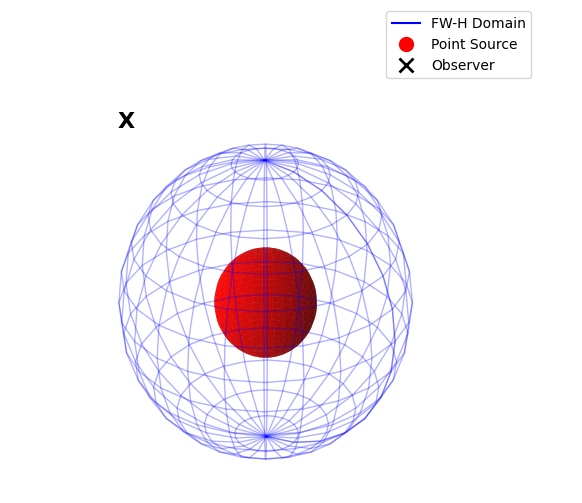
\includegraphics[width=0.9\linewidth]{fig_past_reports/fwh_domain_observer.png}
    \caption{Hybrid domain illustration}
    \label{fig:domain}
\end{figure}

Following this work, CFD will be used as an input to the FW-H code to form a hybrid computational-analytical method, \cite{Kritikos2012, Morgans2004, Thomas2012, Sharma2013}. The Unsteady Reynolds Averaged Navier-Stokes (URANS) framework will be used as it proves effective despite its limitation in capturing high frequency noise from turbulent structures \cite{Fan2025, Mohan2025} from other frameworks such as Detached Eddy Simulation (DES) \cite{Spalart2009} or Large Eddy Simulations (LES). However, for the purpose and limited timeline of this project, URANS is considered sufficient. The point source illustrated in Figure \ref{fig:domain} will later be replaced by the CFD domain.
% The Detached Eddy Simulation (DES) can efficiently resolve noise-emitting turbulent structures \cite{Spalart2009, Fan2025}, as it balances the accuracy of Large Eddy Simulation (LES) in detached flow regions with the lower computational cost of URANS in attached boundary layers. This hybrid DES-FW-H approach will provide a computationally efficient, discrete volumetric source data required for the permeable surface integration.
\clearpage